\documentclass[t]{beamer}

\usepackage[utf8]{inputenc}
\usepackage[english,russian]{babel}

\usepackage{amssymb,amsfonts,amsmath,mathtext}
\usepackage{cite,enumerate,float,indentfirst}
\usepackage{graphicx}
\usepackage{epstopdf}
\epstopdfsetup{suffix=}
\usepackage{tikz}
\usepackage{caption}
\usepackage{subcaption}

\newcommand{\tsetnom}{\tset^\mathrm{nom}}
\newcommand{\brv}[1]{{\left| #1 \right|}}
\newcommand{\brr}[1]{{\left( #1 \right)}}
\newcommand{\brs}[1]{{\left[ #1 \right]}}
\newcommand{\brc}[1]{{\left\{ #1 \right\}}}
\newcommand{\brn}[1]{{\left\lVert #1 \right\rVert}}
\newcommand{\bra}[1]{{\left\langle #1 \right\rangle}}
\newcommand{\brrl}[1]{{\left( #1 \right]}}
\newcommand{\brrr}[1]{{\left[ #1 \right)}}
\newcommand{\under}[2]{{\underset{#2}{\underbrace{#1}}}}
\newcommand{\strm}[1]{\underset{#1}{\rightarrow}}

\makeatletter 
\def\myitem#1{\item[#1] \def\@currentlabel{#1}} 
\makeatother

\usetheme{Darmstadt}

\usefonttheme[onlymath]{serif}

% \definecolor - из пакета xcolor
\definecolor{navyBlue}{RGB}{0,51,153}
\setbeamercolor*{normal text}{fg=navyBlue}
\setbeamercolor*{math text}{fg=black}
% fg = foreground

\beamertemplatenavigationsymbolsempty

\setbeamertemplate{headline}{}

\setbeamertemplate{footline}
{%
\begin{beamercolorbox}{section in head/foot}
  \vskip2pt%
  \hbox to \paperwidth{\insertnavigation{0.95\paperwidth} \hfill% 
    {\scriptsize \bfseries \insertframenumber}\hspace*{3mm}}%
  \vskip2pt
\end{beamercolorbox}%
}


\begin{document}
    \title{Возможность использования искусственных нейронных сетей для решения задач математической физики}
    \author{Кузнецов Игорь Александрович МЕН-490102}
    \date{}
    \begin{frame}
        \titlepage
    \end{frame}

%%%%%%%%%%%%%%%%%%%%%%%%%%%%%%%%%%%%%%%%%%%%%%%%%%%%%%%%%%%%%%%%%%%%%%%%%%%%%%%%%%%%%%%%%%%%%%%%
    \begin{frame}
        \frametitle{Актуальность}
        Physics-informed neural networks (PINN, физически информированные нейронные сети) -- разновидность нейронных сетей, способные решать задачи математической физики. В отличии от классических нейронных сетей, использующих большую выборку данных для обучения, PINN используют уравнения, описывающие физическую систему, что позволяет им обучаться на сравнительно небольших объёмах обучающих данных.
        \begin{figure}
            \center
            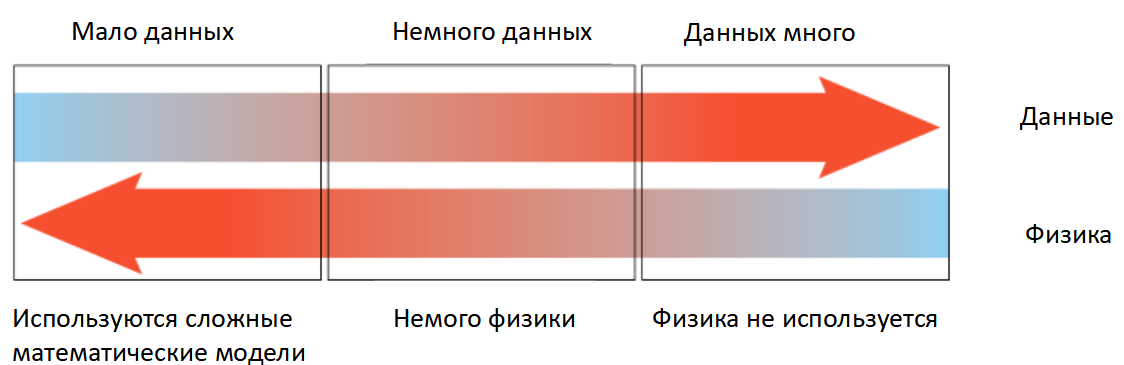
\includegraphics[width=0.85\textwidth]{Данные-Физика.png}
        \end{figure}
        https://www.nature.com/articles/s42254-021-00314-5
    \end{frame}
%%%%%%%%%%%%%%%%%%%%%%%%%%%%%%%%%%%%%%%%%%%%%%%%%%%%%%%%%%%%%%%%%%%%%%%%%%%%%%%%%%%%%%%%%%
    \begin{frame}
        \frametitle{Глубокие нейронные сети}
        Нейрон
        \begin{equation*}
            % f(z, \theta) = h\brr{\sum_{j=1}^p w_j z^j + b} = h(wz+b),
            f(z, \theta) = h(wz+b),
        \end{equation*}
        Глубокая нейронная сеть
        \begin{equation*}
            \begin{aligned}
                % q^{(0, n)} & = h\brr{\sum_{i=1}^p w^{(0,n)}_i z_i + b^{(0,n)}}, n=1,...,N\\
                % q^{(l, n)} & = h\brr{\sum_{i=1}^N w_i^{(l,n)}q^{(l-1,i)}+b^{(l,n)}}, n=1,...,N,\; l=1,...,L-1 \\
                % q^{(L)}    & = {\sum_{i=1}^N w_i^{(L)}q^{(L-1)}+b^{(L)}},
                q^{(0, n)} & = h(w^{(0,n)}z + b^{(0,n)}), n=1,...,N\\
                q^{(l, n)} & = h(w^{(l,n) q^{(l-1,i)} + b^{(l,n)}}), n=1,...,N,\; l=1,...,L-1 \\
                q^{(L)}    & = w^{(L)}q^{(L-1)}+b^{(L)}.
            \end{aligned}
        \end{equation*}
        Обозначим сеть как $\bar{u}(z, \theta) = q^{(L)}$.
        
        Обучение сети $\bar{u}$ на выборке $T = \brc{z_i, u_i}_{i=1}^{N_f}$
        \begin{equation*}
            \theta=\min_\theta\brn{\bar{u}(z_i,\theta)-u_i}, i=1, ..., N_f.
        \end{equation*}
    \end{frame}
%%%%%%%%%%%%%%%%%%%%%%%%%%%%%%%%%%%%%%%%%%%%%%%%%%%%%%%%%%%%%%%%%%%%%%%%%%%%%%%%%%%%%%%%%%
    \begin{frame}
        \frametitle{Устройство PINN}
        Система уравнений
        \begin{equation*}\label{eq:1syst}
            F_j(z, u, \lambda_j) = F_j(z, u, u'_{z^1}, u''_{z^1}, ..., \lambda_j) = 0, z\in\Omega, j=\overline{1,N},
        \end{equation*}
        Граничные условия
        \begin{equation*}\label{eq:1bnd}
            B_k(z_0, u) = 0, z_0 \in \partial\Omega, k=\overline{1,K},
        \end{equation*}
        $\bar{u}$ -- нейронная сеть, аппроксимирующая решение $u$.

        Функция потерь
        \begin{equation*} \label{eq:pinn_loss}
            \begin{aligned}
                MSE & = MSE_f + MSE_b \\
                    & = \sum_{j=1}^N\frac{1}{N_f}\sum_{i=1}^{N_f} F_j^2(z_i, \bar{u}(z_i), \lambda_j) + \sum_{k=1}^{K}\frac{1}{N_b}\sum_{b=1}^{N_b} (\bar{u}(z_b) - u_b)^2.
            \end{aligned}
        \end{equation*}
    \end{frame}
%%%%%%%%%%%%%%%%%%%%%%%%%%%%%%%%%%%%%%%%%%%%%%%%%%%%%%%%%%%%%%%%%%%%%%%%%%%%%%%%%%%%%%%%%%
    \begin{frame}
        \frametitle{Схема работы PINN}
        \begin{figure}
            \center
            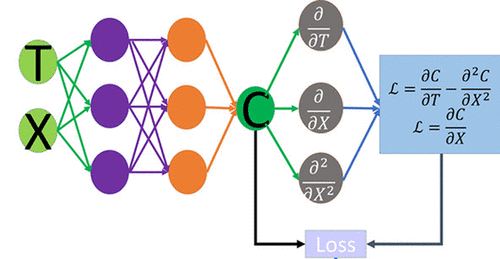
\includegraphics[width=0.8\textwidth]{PINN scheme.png}
        \end{figure}
        https://doi.org/10.1038/s42254-021-00314-5
    \end{frame}
%%%%%%%%%%%%%%%%%%%%%%%%%%%%%%%%%%%%%%%%%%%%%%%%%%%%%%%%%%%%%%%%%%%%%%%%%%%%%%%%%%%%%%%%%%
    \begin{frame}
        \frametitle{Распределение тепла в кольце}
        Уравнение
        \begin{equation*}
            \Delta u = \frac{\partial^2 u}{\partial r} + \frac{1}{r} \frac{\partial u}{\partial r} + \frac{1}{r^2}\frac{\partial^2 u}{\partial \phi^2} = 0.
        \end{equation*}
        Граничные условия
        \begin{equation*}
            \begin{aligned}
                u(1,\phi)= & \cos\phi+\sin\phi+\sin(2\phi)+5\sin(3\phi)+1, \\
                u(2,\phi)= & \sin(2\phi)+\sin(3\phi)+\cos(4\phi).
            \end{aligned}
        \end{equation*}
    \end{frame}
%%%%%%%%%%%%%%%%%%%%%%%%%%%%%%%%%%%%%%%%%%%%%%%%%%%%%%%%%%%%%%%%%%%%%%%%%%%%%%%%%%%%%%%%%%
    \begin{frame}
        \frametitle{Обучение PINN}
        \begin{figure}[htb!]
            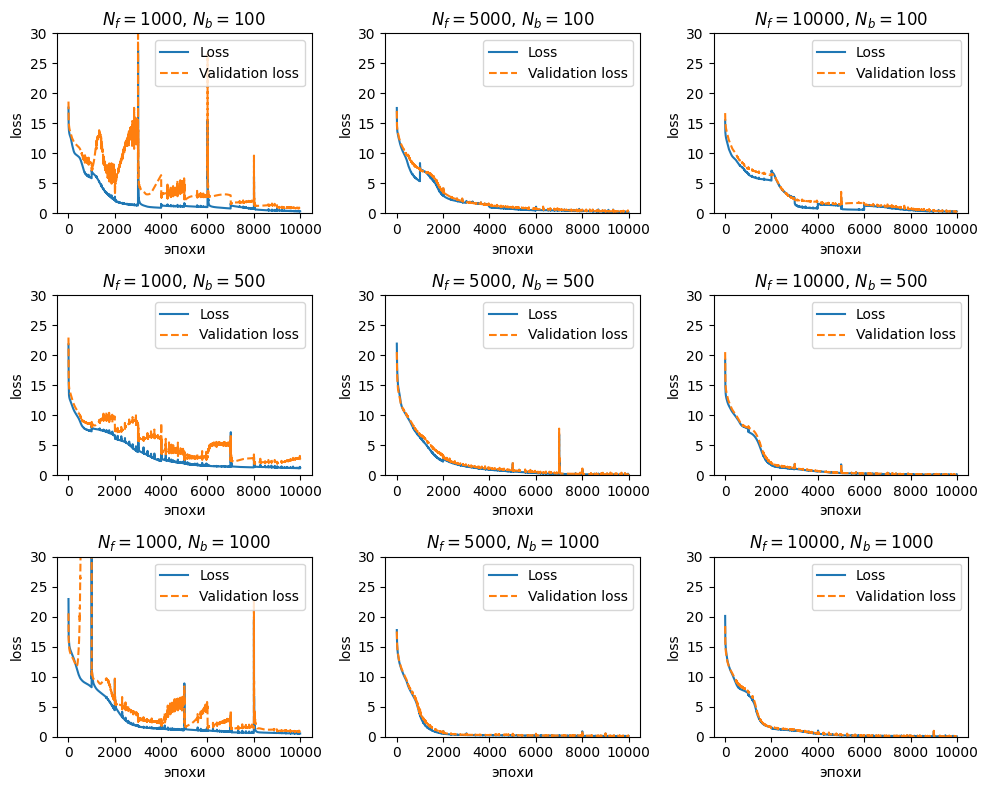
\includegraphics[height=0.7\textwidth]{../plots/termal/loss alt l = (20x4) Nf=[1000, 5000, 10000] Nu=[100, 500, 1000].png}
            % \caption{Графики функций потерь для различных сочетаний $N_f$ и $N_b$, крестиками изображаются результаты валидации в определённые моменты времени}
            % \label{fig:termal_loss}
        \end{figure}
    \end{frame}
%%%%%%%%%%%%%%%%%%%%%%%%%%%%%%%%%%%%%%%%%%%%%%%%%%%%%%%%%%%%%%%%%%%%%%%%%%%%%%%%%%%%%%%%%%
    % \begin{frame}
    %     \frametitle{Решение PINN}
    %     \begin{figure}[ht]
    %         \center
    %         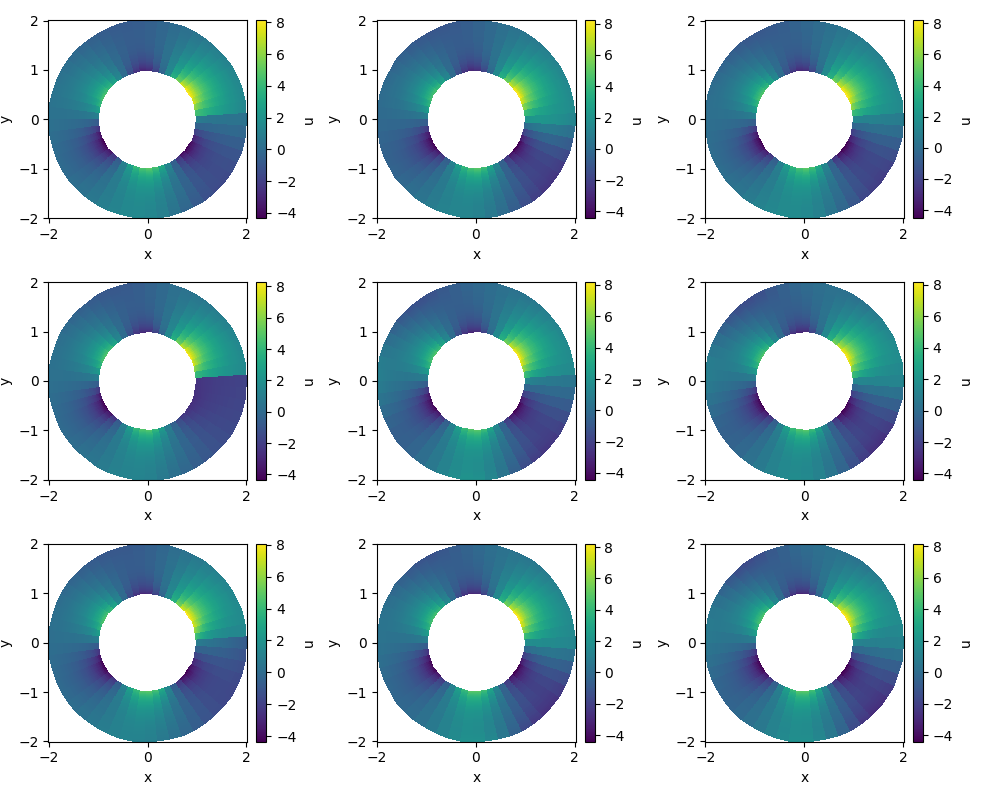
\includegraphics[width=0.8\textwidth]{../plots/termal/solut l = (20x4) Nf=[1000, 5000, 10000] Nu=[100, 500, 1000].png}
    %         % \caption{Решение при различных $N_f$ и $N_b$}
    %         % \label{fig:termal_pred}
    %     \end{figure}
    % \end{frame}
%%%%%%%%%%%%%%%%%%%%%%%%%%%%%%%%%%%%%%%%%%%%%%%%%%%%%%%%%%%%%%%%%%%%%%%%%%%%%%%%%%%%%%%%%%
    \begin{frame}
        \frametitle{Решение PINN и аналитическое решение}
        \begin{figure}[ht]
            \center
            \begin{subfigure}{0.7\textwidth}
                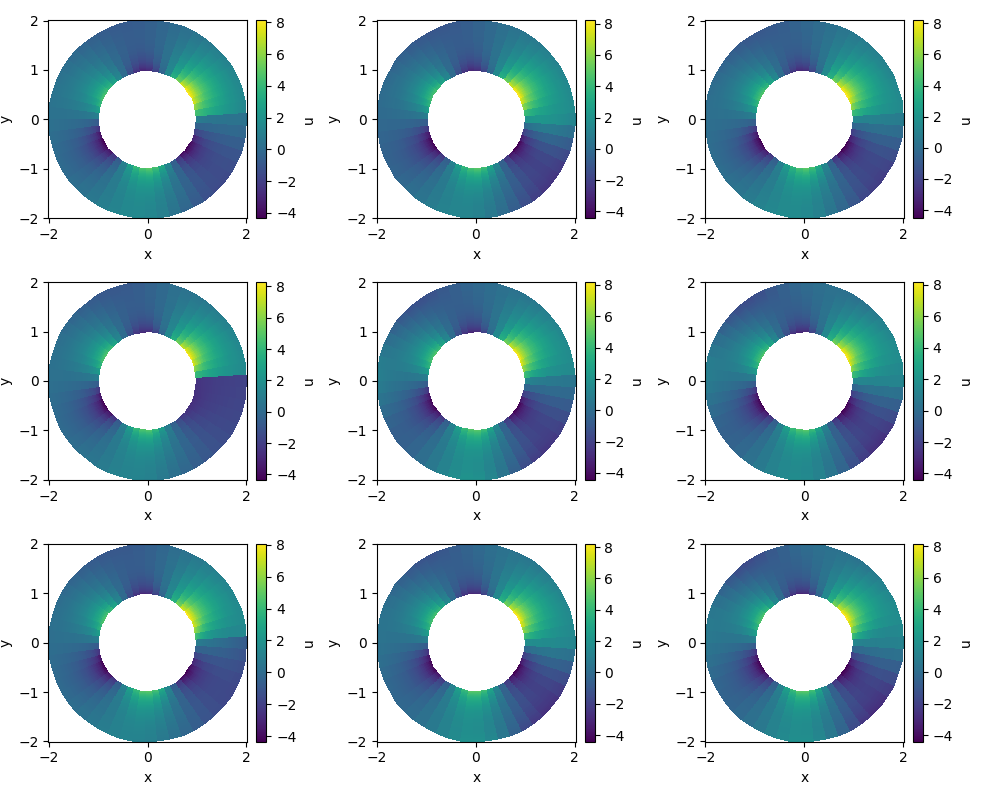
\includegraphics[width=\textwidth]{../plots/termal/solut l = (20x4) Nf=[1000, 5000, 10000] Nu=[100, 500, 1000].png}
                \caption{Решение с PINN}
            \end{subfigure}
            \hfil
            \begin{subfigure}{0.2\textwidth}
                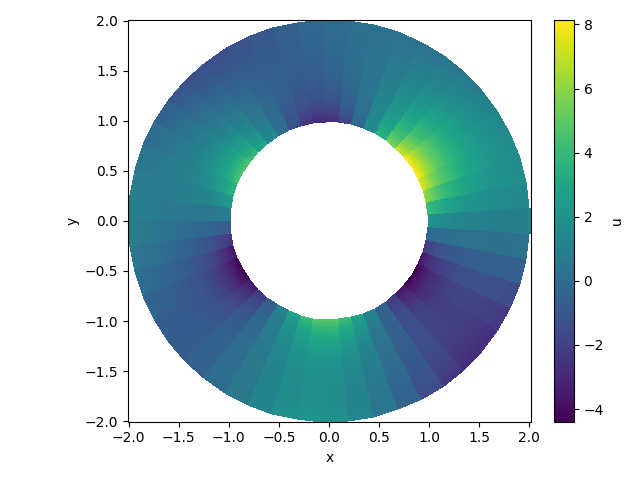
\includegraphics[width=\textwidth]{../plots/termal/solut analit.png}
                \caption{Аналитическое решение}
            \end{subfigure}
        \end{figure}
    \end{frame}
%%%%%%%%%%%%%%%%%%%%%%%%%%%%%%%%%%%%%%%%%%%%%%%%%%%%%%%%%%%%%%%%%%%%%%%%%%%%%%%%%%%%%%%%%%
    % \begin{frame}
    %     \frametitle{Аналитическое решение}
    %     \begin{equation*}\label{eq:termal}
    %         \begin{split}
    %             u(r,\phi) & = 1-\frac{\ln r}{\ln 2}+\brr{\frac{-r}{3}+\frac{4}{3r}}\sin(\phi)\\
    %             &+\brr{\frac{-r}{3}+\frac{4}{3r}}\cos(\phi)+\brr{\frac{r^2}{5}+\frac{4}{5r^2}}\sin(2\phi)\\
    %             &+\brr{\frac{3r^3}{63}+\frac{312}{64r^3}}\sin(3\phi)+\brr{\frac{16r^4}{255}-\frac{16}{255r^4}}\cos(4\phi).
    %         \end{split}
    %     \end{equation*}
    %     \begin{figure}[ht]
    %         \center
    %         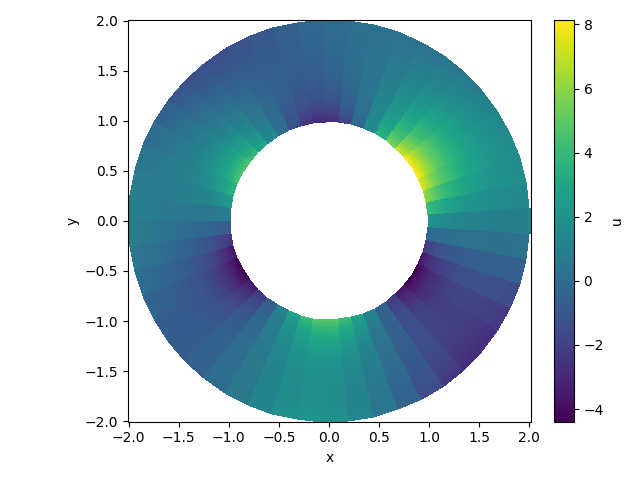
\includegraphics[width=0.4\textwidth]{../plots/termal/solut analit.png}
    %         % \caption{Аналитическое решение}
    %         % \label{fig:termal_analit}
    %     \end{figure}
    % \end{frame}
%%%%%%%%%%%%%%%%%%%%%%%%%%%%%%%%%%%%%%%%%%%%%%%%%%%%%%%%%%%%%%%%%%%%%%%%%%%%%%%%%%%%%%%%%%
    \begin{frame}
        \frametitle{Задача электрокинетики}
        Система
        \begin{equation*}\label{eq:ek_eq}
            \begin{aligned}
                \vec{j}                                             & =
                -D \nabla c - \xi z e c \nabla \Phi + c v,                                    \\
                %
                \frac{\partial c}{\partial t}                                      & =
                -\nabla \cdot\vec{j},                                                         \\
                %
                \nabla^2 \Phi                                       & =
                -4 \pi l_\mathrm{B} k_\mathrm{B}T z c,                                        \\
                %
                \rho \big( \frac{\partial v}{\partial t} + (v \cdot \nabla ) v \big) & =
                -\nabla p_H + \eta \nabla^{2} v - (k_\mathrm{B}T \nabla c + zec \nabla \Phi), \\
                %
                \nabla \cdot v                                      & =
                0.
            \end{aligned}
        \end{equation*}
        Граничные условия
        \begin{equation*}\label{eq:ek_bnd}
            \begin{aligned}
                &c(t, X_l)    = 0.01, c(t, X_r)    = 0.01, c(0, X)      = 0.002        \\
                &v(t, X_l)    = 0, v(t, X_r)    = 0, v(0, X)      = 0            \\
                &\Phi(t, X_l) = -0.05, \Phi(t, X_r) = -0.05, \Phi(0, X)   = -0.009x^2+2.
            \end{aligned}
        \end{equation*}
    \end{frame}
%%%%%%%%%%%%%%%%%%%%%%%%%%%%%%%%%%%%%%%%%%%%%%%%%%%%%%%%%%%%%%%%%%%%%%%%%%%%%%%%%%%%%%%%%%
    \begin{frame}
        \frametitle{Двухмерный случай}
        Обучение
        \begin{figure}[h]
            \begin{subfigure}{0.35\textwidth}
                \center
                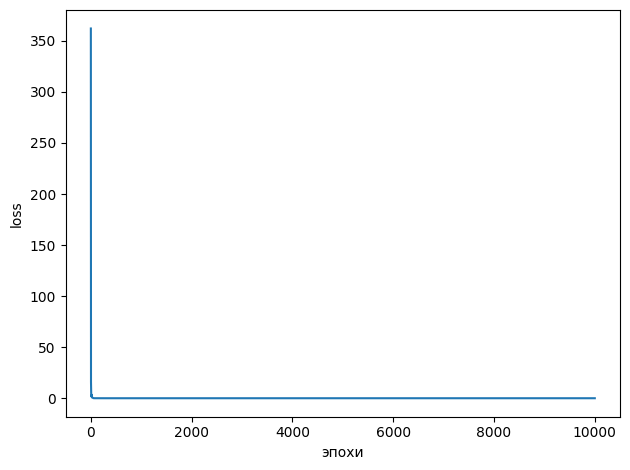
\includegraphics[width=\textwidth]{../plots/ek/2-dim loss 20x4.png}
                % \caption{График обучения за все 10000 эпох}
                % \label{fig:2dloss}
            \end{subfigure}
            \begin{subfigure}{0.35\textwidth}
                \center
                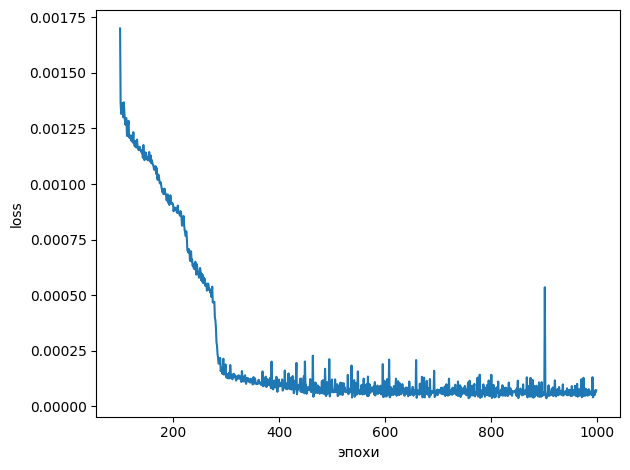
\includegraphics[width=\textwidth]{../plots/ek/2-dim loss trim20x4.png}
                % \caption{График обучения c 100 по 1000 эпохи}
                % \label{fig:2dloss_trim}
            \end{subfigure}
            % \caption{Графики обучения для двухмерного случая электрокинетики для всех эпох и для участка от 100 до 1000}
        \end{figure}
        Результат
        \begin{figure}[H]
            \center
            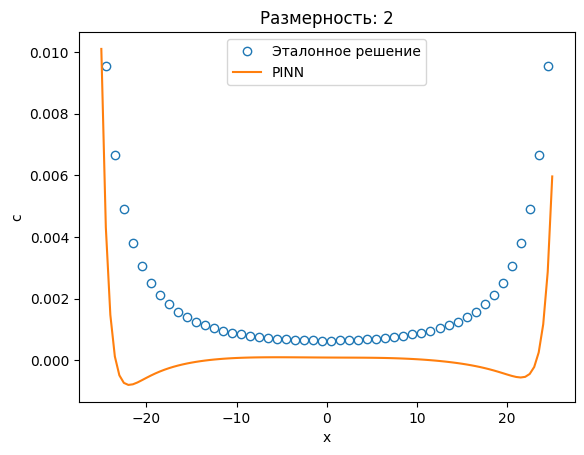
\includegraphics[width=0.4\textwidth]{../plots/ek/2-dim tanh 20x4.png}
            % \caption{Концентрация c для двумерного случая}
            % \label{fig:2dres}
        \end{figure}
    \end{frame}
%%%%%%%%%%%%%%%%%%%%%%%%%%%%%%%%%%%%%%%%%%%%%%%%%%%%%%%%%%%%%%%%%%%%%%%%%%%%%%%%%%%%%%%%%%
    \begin{frame}
        \frametitle{Трёхмерный случай}
        Обучение
        \begin{figure}[h]
            \begin{subfigure}{0.35\textwidth}
                \center
                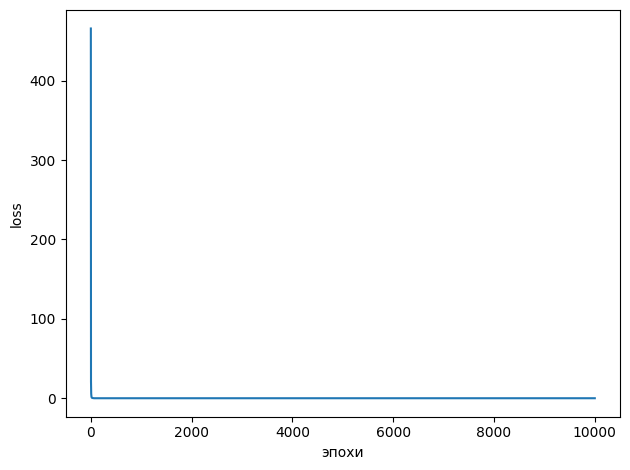
\includegraphics[width=\textwidth]{../plots/ek/3-dim loss 20x4.png}
                % \caption{График обучения за все 10000 эпох}
                % \label{fig:3dloss}
            \end{subfigure}
            \begin{subfigure}{0.35\textwidth}
                \center
                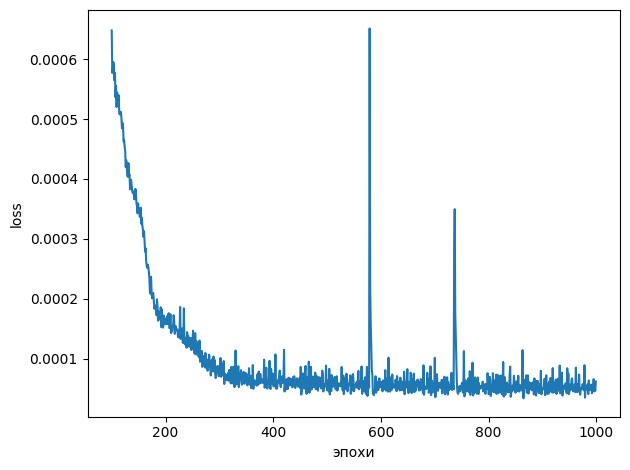
\includegraphics[width=\textwidth]{../plots/ek/3-dim loss trim20x4.png}
                % \caption{График обучения c 100 по 1000 эпохи}
                % \label{fig:3dloss_trim}
            \end{subfigure}
            % \caption{Графики обучения для трёхмерного случая электрокинетики для всех эпох и для участка от 100 до 1000}
        \end{figure}
        Результат
        \begin{figure}[H]
            \center
            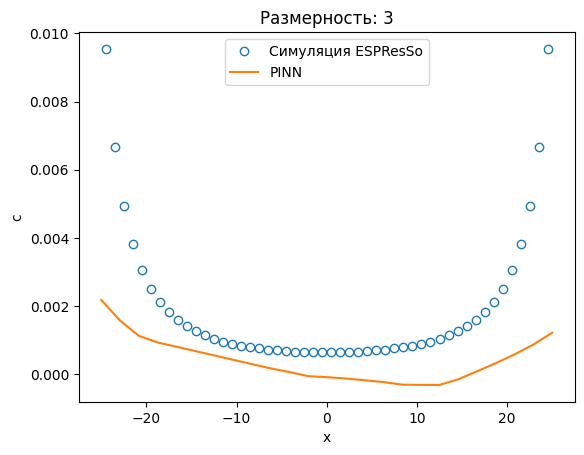
\includegraphics[width=0.4\textwidth]{../plots/ek/3-dim tanh 20x4.png}
            % \caption{Концентрация c для трёхмерного случая}
            % \label{fig:3dres}
        \end{figure}
    \end{frame}
%%%%%%%%%%%%%%%%%%%%%%%%%%%%%%%%%%%%%%%%%%%%%%%%%%%%%%%%%%%%%%%%%%%%%%%%%%%%%%%%%%%%%%%%%%
\begin{frame}
    \frametitle{Результаты работы}
        \begin{itemize}
            \item Для тестовой системы применен метод решения с помощью PINN и получено хорошее согласование с аналитическим решением.
            \item Для системы описывающей задачу электрокинетики в системе щелевой поры применён метод решения с помощью PINN и получено неудовлетворительное согласование и поиск причин - предмет дальнейших исследований.
        \end{itemize}
    \end{frame}
%%%%%%%%%%%%%%%%%%%%%%%%%%%%%%%%%%%%%%%%%%%%%%%%%%%%%%%%%%%%%%%%%%%%%%%%%%%%%%%%%%%%%%%%%%
    \begin{frame}
        \begin{center}
            \vglue100pt
            \Huge Спасибо за внимание
        \end{center}
    \end{frame}
    \end{document}
    